\documentclass[11pt]{article}
\usepackage[bottom=3cm,a4paper]{geometry}
\usepackage{graphicx}
\usepackage{epstopdf}
\usepackage{subcaption}
\usepackage{fancyhdr}

\pagestyle{fancy}
\fancyhf{}
\rhead{Luca Varano \& Tim Fischer}
\lhead{Bits\"ubertragung per Audiosignal}
\cfoot{\thepage}


\begin{document}


\section*{Introduction}
Unser Ziel bei unserem Projekt war es, mithilfe von Matlab Bits FSK-moduliert per Audiosignal zu \"ubermitteln. Daf\"ur haben wir als Grundlage die Ideen aus dem P\&S Bits on Air verwendet.
\section*{Implementation}
Um Bits zu \"ubermitteln durchl\"auft unser Programm folgende Schritte:
\begin{enumerate}

\item \textbf{Startkeys und Endkeys:} Um zu erkennen wann eine \"Ubertragung anf\"angt und endet werden vor und nach dem Bitstream eine bekannte Sequenz von Bits angeh\"angt. 
\item \textbf{Modulation:} Wir haben eine einstellbare FSK-Modulation programmiert, bei der die Ordnung $n$ ausgew\"ahlt werden kann, wobei die Ordnung bedeutet, dass die \"Ubertragung mit $2^n$ Frequenzen modelliert wird. Dabei werden verschiedene Bitfolgen verschiedenen Frequenzen zugewiesen. Bsp.: Bei Ordnung $2$ wird die Sequenz $[0,0] \rightarrow f_{00}$ und $[0,1] \rightarrow f_{01}$ usw.
\item \textbf{\"Ubertragung:} Wir geben den modulierte Bitstream \"uber ein Audiosignal bzw. in unserem Fall ein Kopfh\"orer aus. Empfangen wird das Audiosignal von einem Mikrofon.
\item \textbf{Symbolsynchronisation:} Da der Empf\"anger nicht wissen kann, wann eine Symboldauer anf\"angt muss eine Symbolsynchronisation durchgef\"uhrt werden. Wir haben zwar Anfangsequenzen angeh\"angt, allerdings kann es sein - oder ist sogar sehr wahrscheinlich - das es einen Offset gibt, wobei $\tau_{offset} < \tau_{symbol}$. Dieser Offset wird mit der Symbolsynchronisation eliminiert.
\item \textbf{Demodulation:} Die Demodulation erfolgt analog zur Modulation. Unsere Implementierung beinhaltet eine komplexe Demodulierung mit einer Phasenverschiebung der Empf\"angerfrequenz.
\item \textbf{Rahmensynchronisation:} Schlussendlich werden Anfangs- und End-Bitsequenzen wieder entfernt und die Daten sind \"ubertragen.
\end{enumerate}

\section*{Resultate}
Uns ist es gelungen \texttt{.txt}-Datein \"uber ein Audiosignal zu versenden. Allerdings wird die \"Ubertragung ab Ordnung $3$ bzw. ab 8 Frequenzen ungenau und somit unbrauchbar. Wir vermuten, dass das Rauschen und andere St\"orquellen erheblichen Einfluss haben und deshalb bei vielen unterschiedlichen Frequenzen der Korrelator ungenauer wird.

\pagebreak
\begin{figure}
\centering
\begin{subfigure}{\textwidth}
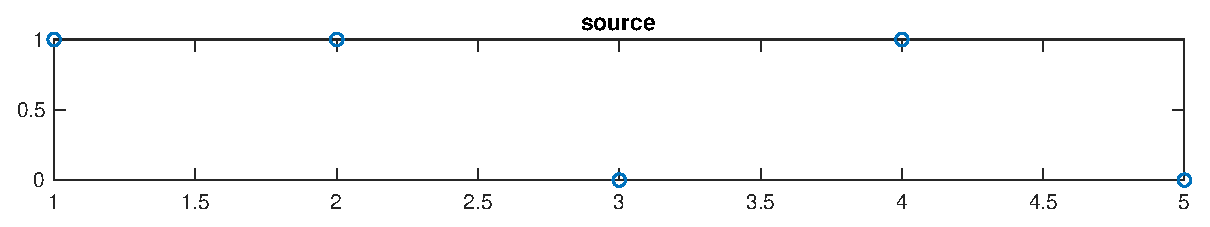
\includegraphics[width=\textwidth]{source.eps}
\caption{Bitstream der zu \"ubermitteln ist}
\end{subfigure}
\begin{subfigure}{\textwidth}
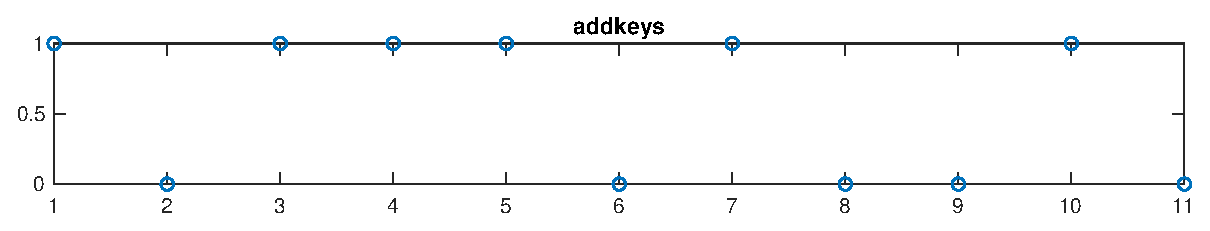
\includegraphics[width=\textwidth]{addkeys.eps}
\caption{Start- und Endsequenz angeh\"angt}
\end{subfigure}
\begin{subfigure}{\textwidth}
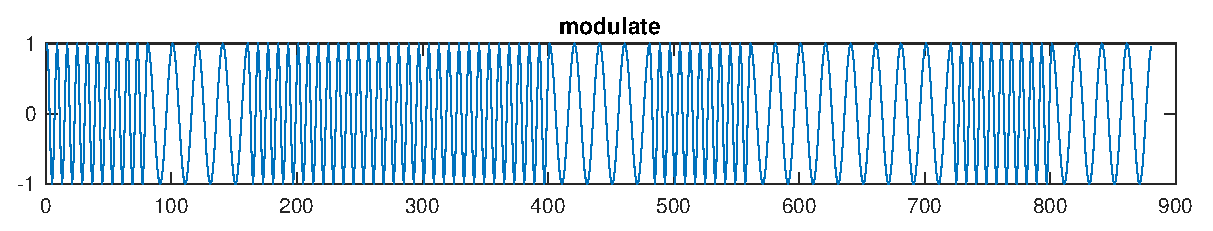
\includegraphics[width=\textwidth]{modulate.eps}
\caption{modulierter Bitstream}
\end{subfigure}
\begin{subfigure}{\textwidth}
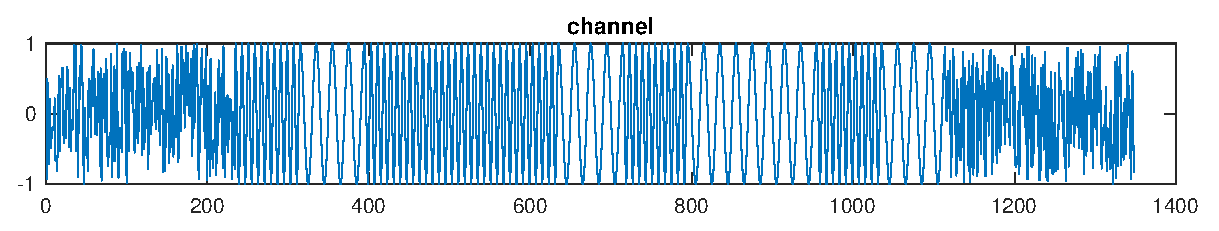
\includegraphics[width=\textwidth]{noisy.eps}
\caption{Signal aus Sicht des Empf\"angers}
\end{subfigure}
\begin{subfigure}{\textwidth}
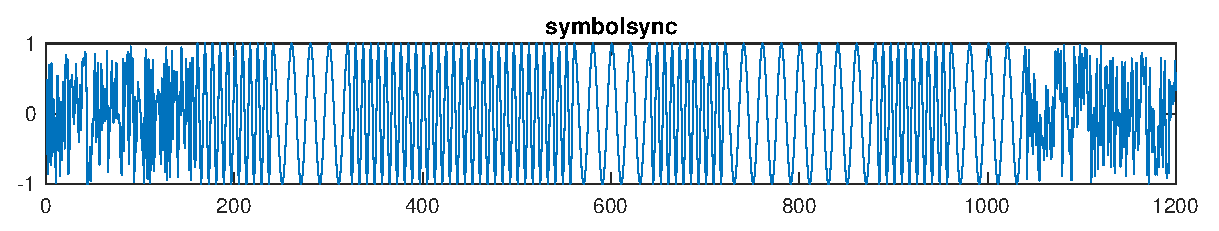
\includegraphics[width=\textwidth]{symbsync.eps}
\caption{Symbolsynchronisation}
\end{subfigure}
\begin{subfigure}{\textwidth}
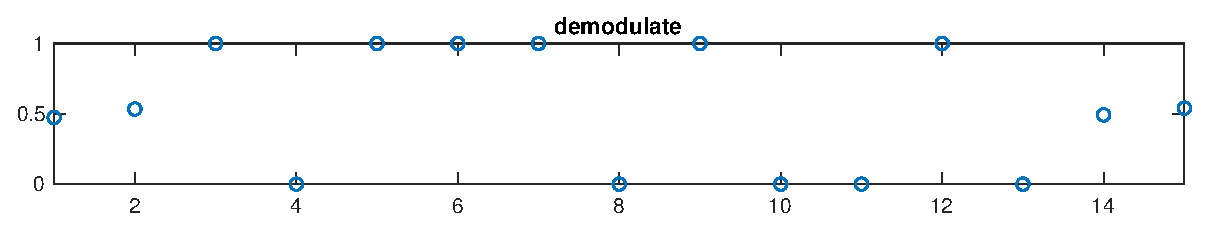
\includegraphics[width=\textwidth]{demodulate.eps}
\caption{Demodulation}
\end{subfigure}
\begin{subfigure}{\textwidth}
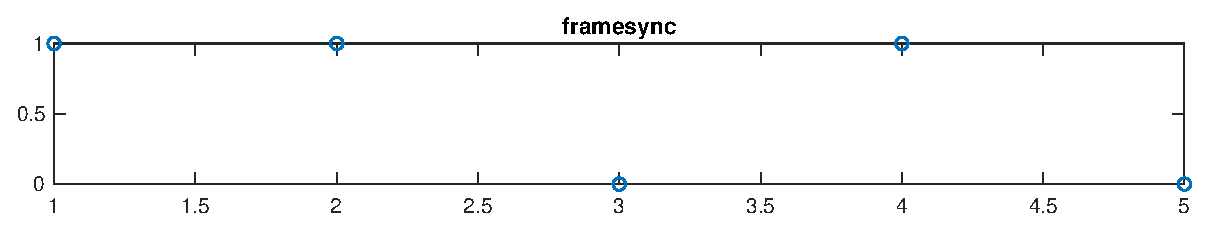
\includegraphics[width=\textwidth]{framesync.eps}
\caption{Rahmensynchronisation}
\end{subfigure}
\end{figure}
\end{document}
